\section*{Supplementary Material}
\subsection*{Stretching parameter $\gamma$}


$\gamma$ is computed with simulations, with the formula $r(t)\propto exp(\gamma dt)\rightarrow\frac{1}{2}ln(r(t))=\gamma t$
if $d=2$ with $r$ being the separation between pairs of particles. $\gamma$ is estimated as the slope of $$\frac{1}{2}\left\langle ln(r(t))\right\rangle =f(t)$$

with $\left\langle ln(r(t))\right\rangle $ being the average obtained from 800 pairs of particles. 

$$\forall t,\left\langle ln(r(t))\right\rangle =\frac{1}{800}\sum_{p=1}^{800}ln(r(\boldsymbol{x}_{1,p}(t)-\boldsymbol{x}_{2,p}(t)))$$ 

where $r(\boldsymbol{x}_{1p}(t)-\boldsymbol{x}_{2p}(t))$ is the distance between a particle $1p$ at position $\boldsymbol{x}_{1p}$ and its counterpart $2p$, initialized with $r(0)=10^{-7}\forall p$ (see
Fig. \ref{fig:gamma_Utot} for $\gamma$ estimates).

\begin{figure}[H]
\begin{centering}
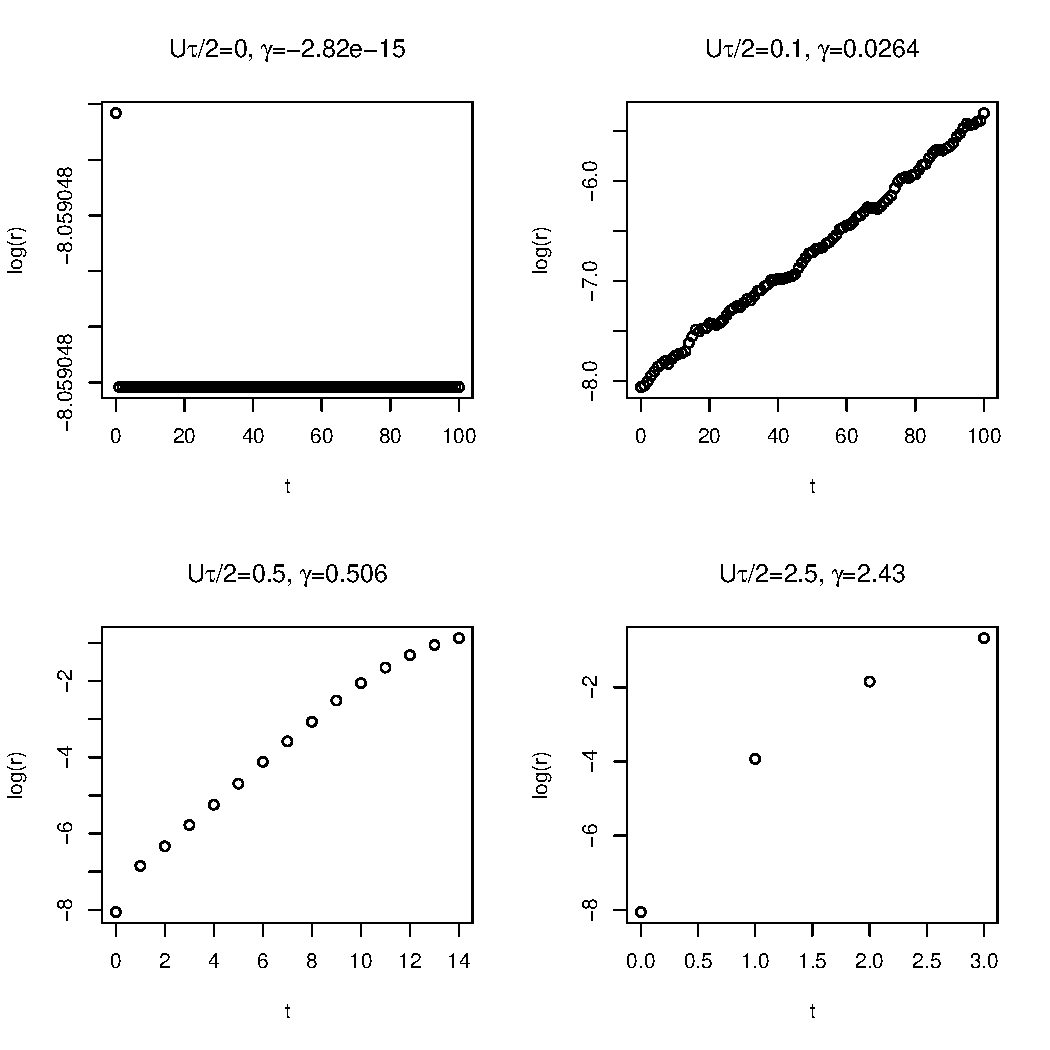
\includegraphics[width=0.95\textwidth]{../code/figure/gamma_for_different_Utot.pdf}
\par\end{centering}
\caption{Estimates of $\gamma$ for different $U\tau/2$\label{fig:gamma_Utot}}
\end{figure}
